\documentclass[a4paper]{scrreprt}

\usepackage[german]{babel}
\usepackage[utf8]{inputenc}
\usepackage[T1]{fontenc}
\usepackage{ae}
\usepackage[bookmarks,bookmarksnumbered]{hyperref}
\usepackage{graphicx}
\usepackage[toc]{glossaries}
\usepackage{tocbasic}
\usepackage{booktabs}
\graphicspath{ {images/} }
\setcounter{secnumdepth}{5}
\makeglossaries
\renewcommand{\arraystretch}{1.5}

\newglossaryentry{android}
{
	name=Android-App, 
	description={Anwendungssoftware für Mobilgeräte mit Android als Betriebssystem}
}   

\begin{document}
    \begin{flushright}
        
\includegraphics[scale = 0.2]{kit-logo.png}\\[0.5cm]
    \end{flushright}
    \vspace*{2cm}

    \begin{center} 
    		\large Praxis der Softwareentwicklung
        \vspace*{1.5cm}

        \textbf{\huge Fridget}
        \vspace*{1cm}

        \textbf{\Large Pflichtenheft}
        \vspace*{2cm}

        Yunjia Chen, Jasmin Jat, Min Hye Park, Alina Shah, Lisa Wang
        \vspace*{1cm}

        27. März 2018
        \vspace*{2.5cm}

        Betreuung: Erik Burger, Sandro Koch\\[0.5cm]
        IPD\\[0.5cm]

        Karlsruher Institut für Technologie
    \end{center}
    \thispagestyle{empty}

    \tableofcontents

    \chapter{Zielbestimmung}
        \section{Musskriterien - KM}
        \begin{table}[h!]
        	\centering
        	\label{my-label}
        	\begin{tabular}{p{2cm}p{12cm}}
        		
        		\multicolumn{2}{c}{\textbf{1 - Erstellen einer WG-Pinnwand}} \\ \hline
        		\centering{[}KM1010{]} & Eine Person muss sich in der App mit einem Google Account registrieren.\\
        		\centering{[}KM1020{]}& Ein Benutzer kann sich mit einem Zugangscode bei einer bestehenden WG-Pinnwand anmelden oder eine neue WG-Pinnwand erstellen.                                 \\
        		\centering{[}KM1030{]}& Beim Erstellen einer neuen WG-Pinnwand gibt der Benutzer der neuen WG-Pinnwand einen Namen.\\ 
        		\centering{[}KM1040{]}& Die Pinnwand ist unterteilt in Frozen Notes und Cool Notes.\\ 
        		\centering{[}KM1050{]}& Die Frozen Notes sind feste, nicht löschbare, bearbeitbare Notizen und werden beim Erstellen der WG generiert.\\ 
        		\centering{[}KM1060{]}& Die Cool Notes sind löschbare, nicht bearbeitbare Notizen und werden vom Benutzer erstellt.\\ 
        		\hline
        	\end{tabular}
        \end{table}
    
    	\vspace{5mm}
    	
    	\begin{table}[h!]
    		\centering
    		\label{my-label}
    		\begin{tabular}{p{2cm}p{12cm}}
    			
    			\multicolumn{2}{c}{\textbf{2 - Interaktion mit der Pinnwand}} \\ \hline
    			\centering{[}KM2010{]} & Der Benutzer kann eine Cool Note mit einer Überschrift und Textinhalt erstellen und löschen.\\
    			\centering{[}KM2020{]}& Der Benutzer kann die Frozen Notes bearbeiten.                                 \\
    			\centering{[}KM2030{]}& Dem Benutzer wird eine Magnetfarbe zugeteilt.\\ 
    			
    			\hline
    		\end{tabular}
    	\end{table}
    
    	\vspace{5mm}
    	
    	\begin{table}[h!]
    		\centering
    		\label{my-label}
    		\begin{tabular}{p{2cm}p{12cm}}
    			
    			\multicolumn{2}{c}{\textbf{3 - Synchronisierung mit dem Server}} \\ \hline
    			\centering{[}KM3010{]} & Der Benutzer kann die App manuell aktualisieren.\\
    			
    			\hline
    		\end{tabular}
    	\end{table}
    
    	\vspace{5mm}
    	
    	\begin{table}[h!]
    		\centering
    		\label{my-label}
    		\begin{tabular}{p{2cm}p{12cm}}
    			
    			\multicolumn{2}{c}{\textbf{4 - App-Menü}} \\ \hline
    			\centering{[}KM4010{]} & Der Benutzer kann eine Liste der Mitglieder und ihre entsprechende Magnetfarbe einsehen.\\
    			\centering{[}KM4020{]}& Der Benutzer kann eine WG verlassen.                               \\
    			\centering{[}KM4030{]}& Die App-Sprache ist Englisch.\\ 
    			
    			\hline
    		\end{tabular}
    	\end{table}
    
    	\vspace{5mm}
    	
    	\begin{table}[h!]
    		\centering
    		\label{my-label}
    		\begin{tabular}{p{2cm}p{12cm}}
    			
    			\multicolumn{2}{c}{\textbf{5 - Lesebestätigung}} \\ \hline
    			\centering{[}KM5010{]} & Der Ersteller sieht, wer seine Cool Notes gelesen hat.\\
    			\centering{[}KM5020{]}& Der Benutzer kann markieren, welche Cool Notes er gelesen hat.                               \\ 
    			
    			\hline
    		\end{tabular}
    	\end{table}
    
    	\vspace{5mm}
    	
    	\begin{table}[h!]
    		\centering
    		\label{my-label}
    		\begin{tabular}{p{2cm}p{12cm}}
    			
    			\multicolumn{2}{c}{\textbf{5 - Push-Benachrichtigung}} \\ \hline
    			\centering{[}KM5010{]} & Alle Mitglieder bekommen für eine neue Cool Note eine Push-Benachrichtigung.\\
    			\centering{[}KM5020{]}& Über die Push-Benachrichtigung gelangt der Benutzer direkt zur neuen Cool Note.                               \\
    			
    			\hline
    		\end{tabular}
    	\end{table}
    	
    	\vspace{1cm}    	

        \section{Wunschkriterien - KW}
		\begin{table}[h!]
			\centering
			\label{my-label}
			\begin{tabular}{p{2cm}p{12cm}}
				
				\multicolumn{2}{c}{\textbf{1 - Taggen}} \\ \hline
				\centering{[}KW1010{]} & Benutzer können in ihrer Cool Note einen oder mehrere Mitglieder taggen.\\
				\centering{[}KW1020{]}& Nur die getaggten Mitglieder bekommen eine Push-Benachrichtigung.                               \\
				\hline
			\end{tabular}
		\end{table}
		
		\vspace{5mm}
		
		\begin{table}[h!]
			\centering
			\label{my-label}
			\begin{tabular}{p{2cm}p{12cm}}
				
				\multicolumn{2}{c}{\textbf{2 - Interaktion mit der Pinnwand}} \\ \hline
				\centering{[}KW2010{]} & Beim Erstellen der Cool Notes kann deren Wichtigkeit durch das Auswählen der Zettelfarbe festgelegt und angezeigt werden.\\
				\centering{[}KW2020{]}& Der Benutzer kann eine Cool Note mit einer Beschreibung und Bildinhalt erstellen und löschen.                              \\
				\centering{[}KW2030{]}& Benutzer können unter Cool Notes Kommentare schreiben.\\ 
				\centering{[}KW2040{]}& Der Benutzer kann eine Cool Note archivieren.\\ 
				\hline
			\end{tabular}
		\end{table}
		
		\vspace{5mm}
		
		\begin{table}[h!]
			\centering
			\label{my-label}
			\begin{tabular}{p{2cm}p{12cm}}
				
				\multicolumn{2}{c}{\textbf{3 - App-Menü}} \\ \hline
				\centering{[}KW3010{]} & Die App kann auf mehrere Sprachen umgestellt werden.\\
				\centering{[}KW3020{]} & Der Benutzer kann archivierte Cool Notes aufrufen.\\
				\hline
			\end{tabular}
		\end{table}
		
		\vspace{5mm}
		
		\begin{table}[h!]
			\centering
			\label{my-label}
			\begin{tabular}{p{2cm}p{12cm}}
				
				\multicolumn{2}{c}{\textbf{4 - Hilfe-Button}} \\ \hline
				\centering{[}KM4010{]} & Beim Drücken des Buttons erscheint ein Tutorial-Overlay.\\
				
				
				\hline
			\end{tabular}
		\end{table}
	
		\vspace{1cm}
		
        \section{Abgrenzungskriterien - KA}
        
        \begin{table}[h!]
        	\centering
        	\label{my-label}
        	\begin{tabular}{p{2cm}p{12cm}}
        		
        		\multicolumn{2}{c}{\textbf{1.3}} \\ \hline
        		\centering{[}KA1010{]} & Die App kann nicht im Querformat benutzt werden.\\
        		\centering{[}KA1020{]}& Keine Browserapp ist geplant.                                 \\
        		\centering{[}KA1030{]}& Man kann nur Mitglieder einer WG sein.\\ 
        		\centering{[}KA1040{]}& Eine WG kann nicht mehr als 15 Mitglieder haben..\\ 
        		\centering{[}KA1050{]}& Cool Notes können nicht bearbeitet werden.\\ 
        		\centering{[}KA1060{]}& Es können nicht mehr als neun Cool Notes pro Pinnwand erstellt werden.\\ 
        		\centering{[}KA1070{]}& Jedes Mitglied kann nur ein Kommentar pro Note schreiben.\\ 
        		\hline
        	\end{tabular}
        \end{table}

    \chapter{Produkteinsatz}
        \section{Anwendungsbereiche}
        Die App ist in einem gemeinsamen Haushalt einsetzbar, um wichtige interne Informationen unmittelbar unter allen Mitbewohnern auszutauschen.
        
        \section{Produktumgebung}
        \begin{tabular}{|l|l|p{.6\textwidth}|}
        	\hline
        	\multicolumn{3}{|l|} {Server} \\
        	\hline
        	Container & Docker & Die Serverseitigen Softwares werden in einem Docker Container verpackt. \\ \hline
        	Webserver & Tomcat & Zum Übertragen von Daten an Client durch HTTP-Anfrage. \\ \hline
        	Datenbank & MySQL & Zum Speichern und Verwalten von Datedn. \\
        	\hline \hline
        	\multicolumn{3}{|l|}{Client} \\
        	\hline
        	Mobiles Betriebssystem & \multicolumn{2}{|l|}{Android 5.1 Lollipop} \\ \hline
        \end{tabular}
        
        \section{Betriebsbedingungen}
        Zur Anmeldung wird ein bereits vorhandenes Google-Konto benötigt. \\
        Zum App-Betrieb wird eine aktive Internetverbindung zum Server benötigt. Ohne eine bestehende Verbindung können weder die Notizen synchronisiert noch Benachrichtigungen erhalten werden.
        
        \section{Zielgruppen}
        Haupt-Zielgruppe der App sind die Personen, die in einer Wohngemeinschaft oder Haushaltsgemeinschaft leben. Ebenfalls kann sie von kleinen Gruppen genutzt werden, die nicht zusammen wohnen, sich jedoch trotzdem verbinden möchten.
        

    \chapter{Produktfunktionen}
    		\section{Grundfunktionen}
    		
    		\section{Optionale Funktionen}
    		
    		\section{Produktleistungen}
    		
    		\section{Qualitäts-Zielbestimmung}

    \chapter{Produktdaten - PD}
    	\begin{table}[h!]
    		\centering
    		\label{my-label}
    		\begin{tabular}{p{2cm}p{12cm}}
    			
    			\multicolumn{2}{c}{\textbf{1 - WG- und Notizendaten}} \\ \hline
    			\centering{[}PD1010{]} & Beim Erstellen einer WG werden der WG-Name und ihr zugehöriger Zugangscode gespeichert.\\
    			\centering{[}PD1020{]}& Beim Beitreten einer WG wird der Benutzer und die zugeteilte Magnetfarbe gespeichert.                                 \\
    			\centering{[}PD1030{]}& Beim Erstellen einer Notiz werden das Erstelldatum, der Benutzer, der die Notiz erstellt hat, die Überschrift und der Textinhalt bis zum Löschen der Notiz gespeichert.\\ 
    			\hline
    		\end{tabular}
    	\end{table}
    
        \vspace{5mm}
        
    	\begin{table}[h!]
    		\centering
    		\label{my-label}
    		\begin{tabular}{p{2cm}p{12cm}}
    			
    			\multicolumn{2}{c}{\textbf{2 - Verlaufdaten}} \\ \hline
    			\centering{[}PD2010{]} & Beim ersten Antippen einer Notiz wird der Benutzer, der die Notiz gelesen hat, bis zum Löschen der Notiz gespeichert.\\ 
    			\hline
    		\end{tabular}
    	\end{table}
    	
    	\vspace{5mm}
    	
    	\begin{table}[h!]
    		\centering
    		\label{my-label}
    		\begin{tabular}{p{2cm}p{12cm}}
    			
    			\multicolumn{2}{c}{\textbf{3 - Anmeldedaten}} \\ \hline
    			\centering{[}PD3010{]} & Beim ersten Anmelden werden die Profildaten (Benutzername, Email-Adresse, Passwort) und die Geräte-ID des Benutzers gespeichert.\\ 
    			\hline
    		\end{tabular}
    	\end{table}
    
    \chapter{Systemmodelle}
        \section{Szenarien}
        
        
        \subsection{Was mache ich mit meinem Kuchen?}
        Max Mustermann wohnt seit 2016 in einer WG. Am Wochenende hatte er Geburtstag und hat von Zuhause Kuchen mitgebracht. In einer großen Dose sind Stücke von seinem Lieblings-Schokokuchen und auch Zitronenkuchen. Er will die Dose nicht in das Gemeinschaftsfach im Kühlschrank legen, da er für sich und seine Freundin den Schokokuchen behalten möchte, aber er möchte nicht noch mal zwei Dosen beschmutzen um die zwei Sorten zu teilen.\\
        Dann erinnert er sich daran, dass, als er mit seinen Kumpels die WG gegründet hat, einer seiner Mitbewohner die WG zu Fridget bekanntgemacht hat. Er kann jetzt in der App eine neue Cool Note erstellen, mit der Überschrift „Kuchen!“ in der er allen seinen Mitbewohnern mitteilen kann, dass es Kuchen zum Essen gibt, aber spezifizieren kann, was gegessen und was überbleiben soll. Er kann außerdem durch die Lesebestätigungen. einsehen dass alle seine Mitbewohner die Notiz gelesen haben.
        \\
        
        \subsection{Medizinischer Notfall}
        Hannah Schmidt ist schon im vierten Semester ihres Studiums und hat endlich eine WG in Laufdistanz zur Uni gefunden. Sie lernt ihre Mitbewohner einen nach dem anderen kennen, und erfährt, dass einer ihrer Mitbewohner eine schwere Allergie hat. Dann fällt ihr ein, wie viele Schwierigkeiten sie hatte mit den Eltern Kontakt aufzunehmen, als ihre ehemalige Mitbewohnerin einen schweren Unfall hatte.\\
        Zum Glück gibt es bei Fridget eine Möglichkeit, durch Frozen Notes Notfallkontakte immer zur Hand zu haben. Die Frozen Notes sind fest, nicht löschbar und klar sichtbar in der App. Hannah lädt die App runter und registriert sich mit ihrem Google Account. Dann kann sie eine WG Pinnwand mit einem einzigartigen Zugangscode generieren und ihre Mitbewohner können damit auf genau diese WG Pinnwand zugreifen. Hannah empfiehlt dann jedem ihrer Mitbewohner, seine Notfallkontakte reinzuschreiben und sie sind immer verfügbar, ohne danach zu suchen oder zu fragen.
        \newpage
        
        \subsection{Ankündigungen}
        Mia wohnt mit ihrem Freund Hans in einer Wohnung zusammen. Als sie nach der Arbeit zuhause ankommt merkt sie, dass der Hausmeister mehrere Ankündigungen an ihre Haustür geklebt hat, unter anderem, ein Zettel mit den Daten der Altpapiersammlung.
        Anstatt diese ganzen Ankündigungen auf Papier kopieren zu müssen, macht Mia Bilder von den Zetteln. Die Bilder kann sie dann mit einer Beschreibung zur Pinnwand hochladen, damit Mia und Hans beide beliebig die Bilder zur Verfügung haben.
        

        \newpage
        \section{Anwendungsfälle}
        	\begin{figure}[h!]
        		\centering
        		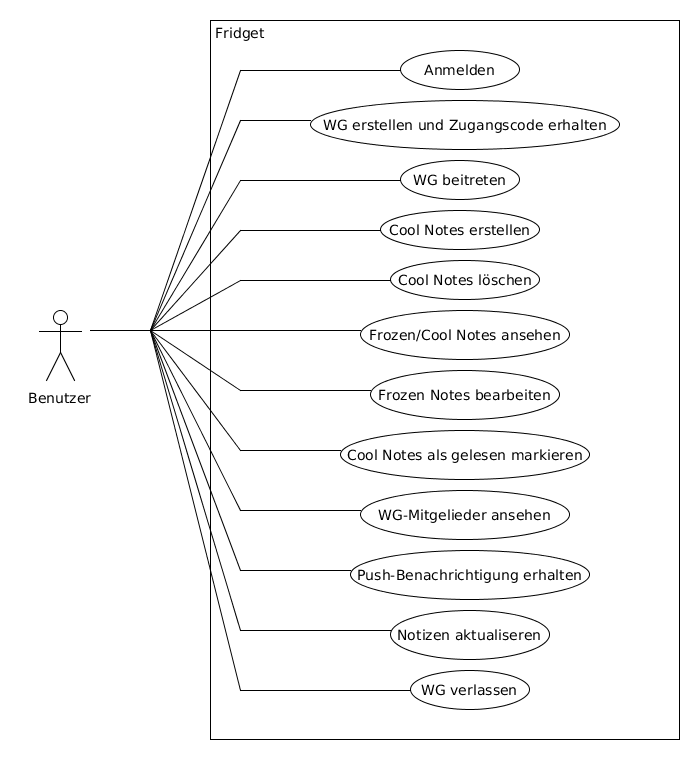
\includegraphics[scale = .6]{anwendungsfalldiagramm.png}
        		\caption{Anwendungsfalldiagramm}
        	\end{figure}
        	
        	\subsection{Anmelden}
        	\textbf{Teilnehmende Akteure}: Benutzer \\
        	\textbf{Eingangsbedingungen}: Der Benutzer hat Fridget installiert und besitzt ein Google-Konto. Das Internet ist verfügbar. \\
        	\textbf{Ausgangsbedingung}: Der Benutzer hat sich angemeldet. \\
        	\textbf{Ereignisfluss}: Benutzer wird angemeldet
        	
        	\subsection{WG erstellen und Zugangscode erhalten}
        	\textbf{Teilnehmende Akteure}: Benutzer \\
        	\textbf{Eingangsbedingungen}: Der Benutzer hat sich angemeldet. Das Internet ist verfügbar. \\
        	\textbf{Ausgangsbedingung}: Ein Zugangscode wurde angezeigt. \\
        	\textbf{Ereignisfluss}: WG wird erstellt $\rightarrow$ Zugangscode wird generiert
        	
        	\subsection{WG beitreten}
        	\textbf{Teilnehmende Akteure}: Benutzer \\
        	\textbf{Eingangsbedingungen}: Der Benutzer hat sich angemeldet und besitzt einen gültigen Zugangscode. Die WG ist nicht voll. Das Internet ist verfügbar. \\
        	\textbf{Ausgangsbedingung}: Der Benutzer ist einer WG beigetreten. \\
        	\textbf{Ereignisfluss}: WG wird beigetreten
        	
        	\subsection{Cool Notes erstellen}
        	\textbf{Teilnehmende Akteure}: Benutzer \\
        	\textbf{Eingangsbedingungen}: Der Benutzer hat sich angemeldet und ist einer WG beigetreten. Die Pinnwand ist nicht voll und keiner erstellt gerade die letzte Cool Note. Das Internet ist verfügbar. \\
        	\textbf{Ausgangsbedingung}: Der Benutzer hat das Erstellen bestätigt. \\
        	\textbf{Ereignisfluss}: Cool Note wird erstellt
        	
        	\subsection{Cool Notes löschen}
        	\textbf{Teilnehmende Akteure}: Benutzer \\
        	\textbf{Eingangsbedingungen}: Der Benutzer hat eine Cool Note, die nicht von ihm erstellt wurde, geöffnet. Keiner liest gerade dieselbe Cool Note. Das Internet ist verfügbar. \\
        	\textbf{Ausgangsbedingung}: Der Benutzer hat das Löschen bestätigt. \\
        	\textbf{Ereignisfluss}: Cool Note wird gelöscht
        	
        	\subsection{Frozen/Cool Notes ansehen}
        	\textbf{Teilnehmende Akteure}: Benutzer \\
        	\textbf{Eingangsbedingungen}: Der Benutzer hat sich angemeldet und ist einer WG beigetreten. Die Pinnwand ist nicht leer. Das Internet ist verfügbar. \\
        	\textbf{Ausgangsbedingung}: Eine Frozen/Cool Note wurde angezeigt. \\
        	\textbf{Ereignisfluss}: Frozen/Cool Note wird geöffnet $\rightarrow$ Frozen/Cool Note wird angesehen
        	
        	\subsection{Frozen Notes bearbeiten}
        	\textbf{Teilnehmende Akteure}: Benutzer \\
        	\textbf{Eingangsbedingungen}: Der Benutzer hat eine Frozen Note geöffnet. Keiner bearbeitet gerade dieselbe Frozen Note. Das Internet ist verfügbar. \\
        	\textbf{Ausgangsbedingung}: Der Benutzer hat das Bearbeiten bestätigt. \\
        	\textbf{Ereignisfluss}: Frozen Note wird bearbeitet
        	
        	\subsection{Cool Notes als gelesen markieren}
        	\textbf{Teilnehmende Akteure}: Benutzer \\
        	\textbf{Eingangsbedingungen}: Der Benutzer hat eine Cool Note, die nicht von ihm erstellt wurde, geöffnet. Die Cool Note wurde noch nicht als gelesen markiert. Das Internet ist verfügbar. \\
        	\textbf{Ausgangsbedingung}: Der Benutzer hat die Cool Note als gelesen markiert. \\
        	\textbf{Ereignisfluss}: Cool Note wird markiert
        	
        	\subsection{WG-Mitgelieder ansehen}
        	\textbf{Teilnehmende Akteure}: Benutzer \\
        	\textbf{Eingangsbedingungen}: Der Benutzer hat sich angemeldet und ist einer WG beigetreten. Das Internet ist verfügbar. \\
        	\textbf{Ausgangsbedingung}: Die WG-Mitgelieder werden angezeigt. \\
        	\textbf{Ereignisfluss}: WG-Mitgelieder-View wird geöffnet $\rightarrow$ WG-Mitgelieder werden angesehen
        	
        	\subsection{Push-Benachrichtigung erhalten}
        	\textbf{Teilnehmende Akteure}: Benutzer \\
        	\textbf{Eingangsbedingungen}: Der Benutzer hat sich angemeldet und ist einer WG beigetreten. Der Benutzer hat ``Push-Benachrichtigung'' von Fridget aktiviert. Das Internet ist verfügbar. \\
        	\textbf{Ausgangsbedingung}: Die Push-Benachrichtigung wird auf den Geräten des Benutzers angezeigt. \\
        	\textbf{Ereignisfluss}: Neue Cool Note wird erstellt $\rightarrow$ Push-Benachrichtigung wird erhalten
        	
        	\subsection{Notizen/Mitglieder aktualisieren}
        	\textbf{Teilnehmende Akteure}: Benutzer \\
        	\textbf{Eingangsbedingungen}: Der Benutzer hat sich angemeldet und ist einer WG beigetreten. Das Internet ist verfügbar. \\
        	\textbf{Ausgangsbedingung}: Die Änderungen von Notizen/Mitgliedern wurden mit dem Server synchronisiert. \\
        	\textbf{Ereignisfluss}: Pinnwand wird nach unten gewischt $\rightarrow$ Notizen/Mitglieder werden aktualisiert
        	
        	\subsection{WG verlassen}
        	\textbf{Teilnehmende Akteure}: Benutzer \\
        	\textbf{Eingangsbedingungen}: Der Benutzer hat sich angemeldet und ist einer WG beigetreten. Das Internet ist verfügbar. \\
        	\textbf{Ausgangsbedingung}: Der Benutzer hat das Verlassen der WG bestätigt. \\
        	\textbf{Ereignisfluss}: WG wird verlassen
        	
        	\newpage
        \section{Bedienoberfläche}
        
        \begin{figure}[h]
        	\begin{minipage}[b]{0.4\linewidth}
        		
        		\flushright
        		\centering
        		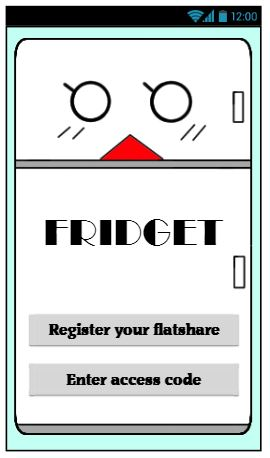
\includegraphics[width=0.7\textwidth]{fridget_start.JPG}
        		\caption{default}
        		\label{fig:figure1}
        	\end{minipage}
        	\hspace{0.5cm}
        	\begin{minipage}[b]{0.55\linewidth}
        		\flushleft
        		{[}S01{]} Startbildschirm 
        		
        		Beschreibung: \\
        		Startbildschirm der App. Dieser erscheint nachdem man sich mit dem Google-Account angemeldet hat. Man hat die Wahl zwischen WG erstellen und Zugangscode eingeben, um einer bereits vorhandenen WG beizutreten.
        		\\
        		Elemente:
        		\begin{itemize}
        		\renewcommand\labelitemi{--}
        		\item Button zum Erstellen der WG
        		\item Button zum Eingeben des Zugangscodes
        		\end{itemize}
        		
        		Verwendung:\\
        		Durch das Tippen auf den oberen Button
        		kann man eine WG erstellen, indem man ihr
        		einen Namen gibt {[}S02{]}.\\
        		Durch das Tippen auf den unteren Button kann
        		man den Zugangscode eingeben {[}S04{]}, den man zuvor vom WG-Ersteller extern erhalten 
        		hat.
        		
        	\end{minipage}
        \end{figure}
    
    	\begin{figure}[h!]
    		\begin{minipage}[t]{0.4\linewidth}
    			\flushright
    			\centering
    			\vspace{9mm}
    			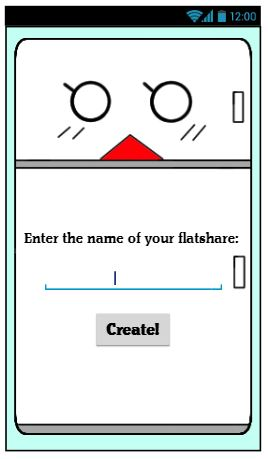
\includegraphics[width=0.7\textwidth]{fridget_nameenter.JPG}
    			\caption{default}
    			\label{fig:figure1}
    		\end{minipage}
    		\hspace{0.5cm}
    		\begin{minipage}[t]{0.55\linewidth}
    			\flushleft
    			\vspace{9mm}
    			{[}S02{]} Namensgebung
    			
    			Beschreibung: \\
    			View zur Namesgebung einer WG.
    			\\
    			Elemente:
    			\begin{itemize}
    				\renewcommand\labelitemi{--}
    				\item Textfeld zum Eingeben des Namens
    				\item Button zum endgültigen Erstellen der WG
    				
    			\end{itemize}
    			
    			Verwendung:\\
    			Durch das Tippen auf das Textfeld kann man
    			den Namen der WG eingeben.
    			Durch das Tippen auf den Button wird ein 
    			zufälliger aber einzigartiger Zugangscode 
    			generiert und ausgegeben {[}S03{]}.
    			
    			
    			
    		\end{minipage}
    	\end{figure}

    \chapter{Testfälle}
    
    \chapter{Entwicklungsumgebung}

	\chapter{Glossar}
	
    \glsaddall
    \printglossaries

    \listoffigures

\end{document}